\chapter{Pixelové detektory radiace a vyčítací zařízení}	% + pro pixelové detektory
\label{kap:2}
Mezi možnosti detekovat ionizující záření patří mimo jiné, použití pixelových detektorů. Pomocí pixelových detektorů, konkrétněji hybridních pixelových detektorů, jsme schopni detailně změřit ionizující záření. V dalších částech této kapitoly bude popsána obecná činnost a princip detekce radiace pixelových detektorů. V části \ref{Timepix2}, bude konkrétně popsán detektor z rodiny Timepix \cite{Llopart}, detektor Timepix 2 \cite{tpx2_manual}. 

\section{Princip činnosti pixelových detektorů}
\label{kap:2.1}
V této části bude popsán obecný princip činnosti pixelových detektorů, který je společný pro detektory radiace z rodiny Timepix \cite{Llopart}, vyvíjenými pod záštitou CERN Medpipix Collaboration \cite{Medpix}. Pixelový detektor, přesněji hybridní pixelový detektor se skládá ze dvou oddělitelných částí, ze senzorové vrstvy a vrstvy s vyčítací elektronikou viz. obrázek \ref{fig:Timepix}. Právě toto rozdělení na senzorovou a vyčítací část označuje název hybridní detektor.
\par Senzorová vrstva je tvořena polovodičovým materiálem. Důležitými parametry senzorové vrstvy jsou typ polovodičového materiálu a její tloušťka. Nejčastěji používané materiály jsou $\text{Si}$, $\text{CdTe}$ a $\text{GaAs}$. Na senzorovou vrstvu je připojené vysoké napětí, označované jako \textit{bias voltage}. Toto vysoké napětí zajistí vyprázdnění oblasti v polovodičové struktuře senzorové vrstvy. Pokud částice ionizujícího záření interaguje v senzorové vrstvě, dojde k vytvoření náboje. Tento náboj je dále zpracován vyčítací elektronikou která je pomocí technologie nazývající se \textit{bump bond}, připojena k senzorové vrstvě.
\par Vyčítací vrstva (ASIC) je rozdělena na 256x256 individuálních pixelů. Každý pixel obsahuje potřebnou elektroniku ke zpracovaní náboje, vzniklého v senzorové vrstvě. Detailnější popis zpracování analogového náboje na úrovni jednotlivých pixelů, bude popsán pro konkrétní pixelový detektor Timepix 2 v části \ref{Timepix2}. Po analogovém zpracování signálu následuje digitální zpracování, poté je digitální signál převeden na výstupní plošky. Vyčítací vrstva je pomocí \textit{wire bond} technologie připojena k desce plošných spojů. Signály vedoucí z pixelových detektorů jsou následně zpracovány vyčítacím zařízením. Druhy vyčítacích zařízní budou popsány v části \ref{Vycitaci zarizeni}.
 \begin{figure}[h!]
 	\centering
 	\captionsetup{justification=centering}
 	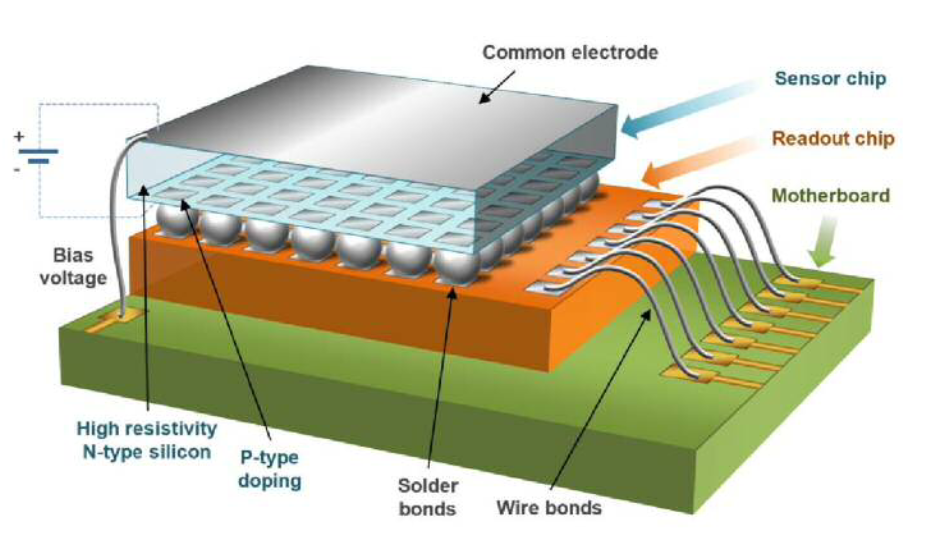
\includegraphics[scale=0.55]{Timepix.png}
 	\caption{Rozložení hybridního pixelového detektoru Timepix \cite{Platkevic}} 
 	\label{fig:Timepix}
 \end{figure}	

\section{Vyčítací zařízení pro pixelové detektory}
\label{Vycitaci zarizeni}
Každý pixelový detektor z rodiny detektorů Timepix \cite{Llopart}, má specifické požadavky pro návrh vyčítacího zařízení. Základními požadavky jakými jsou napájecí napětí detektoru a komunikační rozhraní s detektorem, musí být vždy splněny aby bylo možné spolehlivě komunikovat s pixelovým detektorem. Vyčítacích zařízení existuje celá řada. V této práci, respektive v následujících částech bude popsán návrh miniaturizovaného vyčítacího rozhraní. Pokusím se zde tedy uvést příklady miniaturizovaných zařízení.
\subsection{USB Lite}
Dosud nejmenším vyčítacím zařízení rodiny detektorů Timepix \cite{Llopart}, je zařízení \textit{USB Lite} \cite{usb_lite}, viz. obrázek \ref{fig:usb_lite}. Toto zařízení umožňuje komunikovat s detektorem Medipix 2 \cite{Medpix2}. Rozměry zařízení jsou 60x15 mm. Rychlost vyčítání snímků je 4 fps a spotřeba zařízení je menší než 2 W \cite{usb_lite}.
 \begin{figure}[h!]
	\centering
	\captionsetup{justification=centering}
	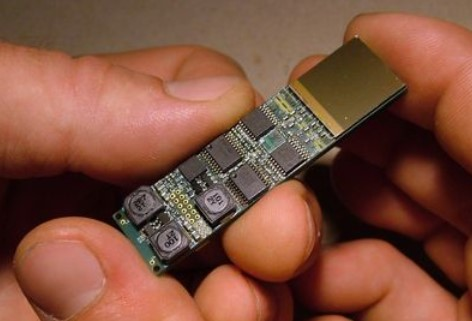
\includegraphics[scale=0.55]{usb_lite.jpg}
	\caption{Vyčítací zařízení \textit{USB lite}} 
	\label{fig:usb_lite}
\end{figure}	

\subsection{MiniPIX SPRINTER}
Vyčítací zařízení MiniPIX SPRINTER je vyvíjeno společností ADVACAM, zařízení je možné vidět na obrázku \ref{fig:sprinter}. Toto zařízení umožňuje komunikovat s detektorem Timepix 2 \cite{tpx2_manual}. Rozměry zařízení jsou 50x21x14 mm. Rychlost vyčítání snímků je 99 \cite{Advacam}.
\begin{figure}[h!]
	\centering
	\captionsetup{justification=centering}
	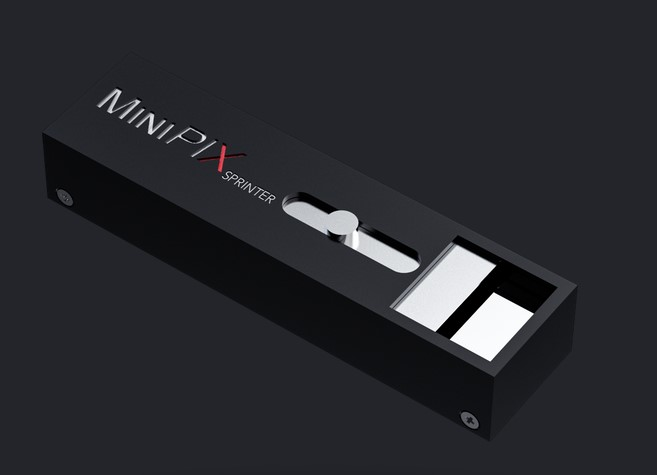
\includegraphics[scale=0.55]{sprinter.jpg}
	\caption{Vyčítací zařízení MiniPIX SPRINTER} 
	\label{fig:sprinter}
\end{figure}	

\subsection{Katherine pro Timepix 2} %katherine zminena protoze modularita
Posledním uvedeným tipem vyčítacího zařízení je zařízení Kathrine pro Timepix 2, které můžete vidět na obrázku \ref{fig:Katherine2}. Toto vyčítací zařízní se od předchozích dvou uvedených liší ve velikosti a maximalní rychlosti komunikace. Zařízení se skládá ze dvou částí. Samotným vyčítacím zařízením, na obrázku \ref{fig:Katherine2} vpravo a takzvaným \textit{chipboardem}, na obrázku \ref{fig:Katherine2} vlevo. Část chipboardu obsahuje detektor Timepix 2 a napájecí zdroje potřebné pro provoz detektoru. Dále jsou ze propojeny signály z konektoru od vyčítacího zařízení po samotný Timepix 2. Výhodou tohoto modulárního zapojení je možnost modifikace chipboardové části, bez nutnosti změn na straně vyčítacího zařízení. Tedy existuje možnost k jednomu vyčítacímu zařízení, připojit různé chipboardy. Parametry samotného vyčítacího zařízení jsou následující. Rozměry 100x80x28 mm, rychlost vyčítaní až 3.2 Gbps \cite{Burian_2020}.
\begin{figure}[h!]
	\centering
	\captionsetup{justification=centering}
	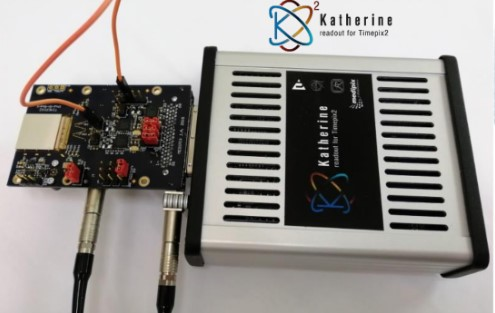
\includegraphics[scale=0.75]{Katherine2.jpg}
	\caption{Vyčítací zařízení Katherine pro Timepix 2 \cite{Burian_2020}} 
	\label{fig:Katherine2}
\end{figure}	

%%%
%%%%%%%%%%%%%%%%%%%%%%%%%%%

\section{Timepix 2}
% v podstatě technická dokumentace Timepix 2, plus konkretni pozadavky pro provoz
\label{Timepix2}
V předchozí části \ref{kap:2.1}, byly popsány obecné vlastnosti detektoru a základní principy detekce ionizujícího záření. V této kapitole bude detailněji popsán konkrétní detektor, detektor Timepix 2 \cite{tpx2_manual}. Detektor byl vyvinut pod záštitou CERN Medpipix Collaboration \cite{Medpix}. Timepix 2 patří do rodiny detektorů Timepix. Prvním z rodiny detektorů byl detektor Timepix \cite{Llopart}, následně to popořadě byly detektory Timepix 3 \cite{Timepix3}, Timepix 2 \cite{tpx2_manual}, \cite{Timepix2} a nejnovějším detektorem je Timepix 4 \cite{Timepix4}. Detektor Timepix 2 je zobrazen na obrázku \ref{fig:Timepix2}.
\begin{figure}[h!]
	\centering
	\captionsetup{justification=centering}
	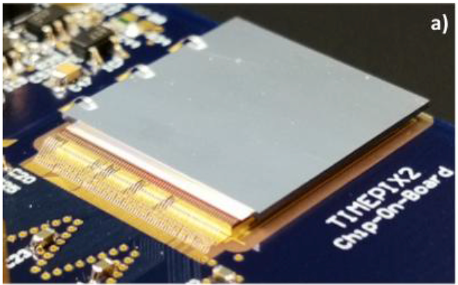
\includegraphics[scale=0.80]{Timepix2.png}
	\caption{Detektor Timepix 2 \cite{Timepix2}} 
	\label{fig:Timepix2}
\end{figure}	

\subsection{Analogová část}	 %todo upravit
Každý pixel z matice 256x256 pixelů má vlastní analogovou částí. Jak bylo zmíněno v kapitole \ref{kap:2}, pokud částice interaguje na senzorové vrstvě dojde k vytvoření nábojového impulsu. Tento náboj je díky připojenému napětí přitažen k elektrodám. Tento náboj může být charakterizován jako Diracův proudový impuls. Integrací Diracovo proudového impulsu dostaneme celkový generovaný náboj Q. Diracův impuls je naintegrován do malého kapacitoru Cf. Poté na výstupu CSA je v ideálním případě napěťový skok s amplitudou Q/Cf viz. \ref{fig:pixel_frontend}. Výstupní puls je poté porovnán s prahovou úrovní. Nastavením prahové úrovně lze eliminovat zbytkový proud, takzvaný \textit{leakage current}, závěrného směru polovodičové struktury, který zde vznikl kvůli připojenému vysokému napětí. Pokud je signál větší než daná nastavená úroveň, je inkrementován digitální čítač \cite{Llopart}. Každý diskriminátor obsahuje 5-bitový DAC převodník. Tento 5 bitový DAC převodník umožňuje nastavit úroveň detekovatelného signálu pro každý pixel individuálně a tím eliminovat šum. Uuspořádaní pro analogovou část lze vidět na obrázku \ref{fig:tpx2_cel}, kde je zobrazeno uspořádání jednoho pixelu detektoru Medipix 2.
\begin{figure}[h!]
	\begin{subfigure}{0.5\textwidth}
	\centering
	\captionsetup{justification=centering}
	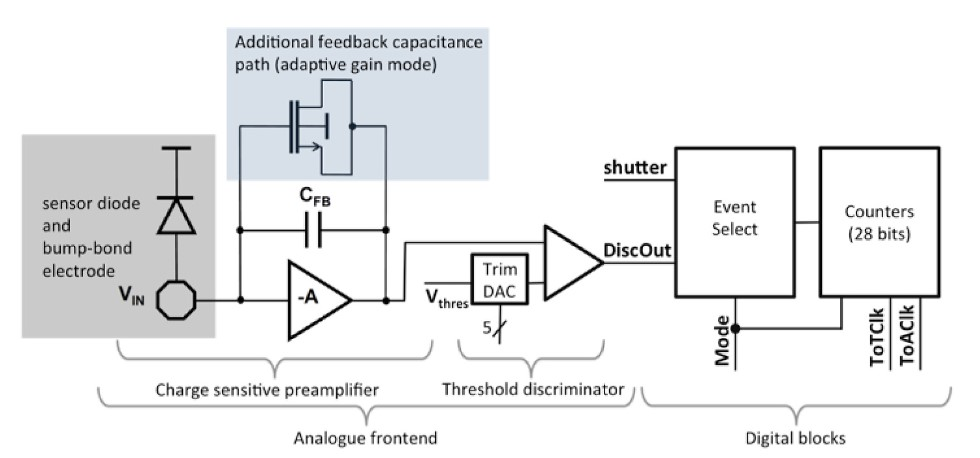
\includegraphics[scale=0.70]{tpx2_cel.jpg}
	\caption{Uspořádání jednoho pixelu} 
	\label{fig:tpx2_cel}
	\end{subfigure}
	\begin{subfigure}{0.5\textwidth}
		\centering
		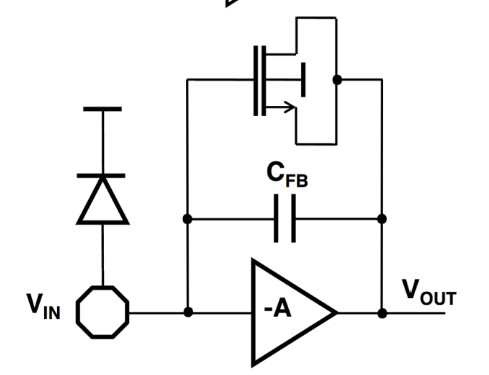
\includegraphics[scale=0.50]{pixel_frontend.jpg}
		\caption{První stupeň zpracování signálu, CSA}
		\label{fig:pixel_frontend}
	\end{subfigure}
	\caption{Zpracování signálu na úrovni pixelů}
	\label{fig:zpracování signálu}
\end{figure}

\subsection{Digitální část}
Každý pixel obsahuje čtyři digitální čítače typu LSFR. Každý n-bitový čítač generuje $2^n$ pseoudonáhodných čísel. V případě Timepix 2 každý pixel obsahuje dva 10-bitové (A,B) a dva 4-bitové (C,D) čítače. Například tedy 14-bitový čítač vznikne kombinací 10-bitového a 4-bitového čítače. Odpovídající 14-bitová hodnota je poté viz \ref{eq:1}. Celkem tedy pro každý pixel lze využít 28-bitů. Tyto čítače mouhou pracovat v různých módech. Tyto módy budou probrány v další části.
\begin{equation}
	14-bit = (hodnota_{4-bit} \cross 2^{10}) + hodnota_{10-bit}
	\label{eq:1}
\end{equation}

Jak bylo zmíněno výše. Každý z digitálních čítačů může být nakonfigurován do jiného módu. Pro Timepix 2 jsou to následující módy \ref{fig:modes}. 
\begin{itemize}
	\item \textbf{Time over Threshold} (ToT): Čítač je inkrementován při každým hodinovým pulsu, kdy je signál nad nastavenou prahovou úrovní
	\item \textbf{Time of Arrival} (ToA): Čítač je inkrementován při každým hodinovým pulsu, kdy signál překročí nastavenou úroveň a inkrementuje se až do konce akvizice.
	\item \textbf{Coutnig mode}: Čítač je inkrementován pokud signál překročí dvakrát nastavený práh, viz. obrázek \ref{fig:modes} 
\end{itemize}
\begin{figure}[h!]
	\centering
	\captionsetup{justification=centering}
	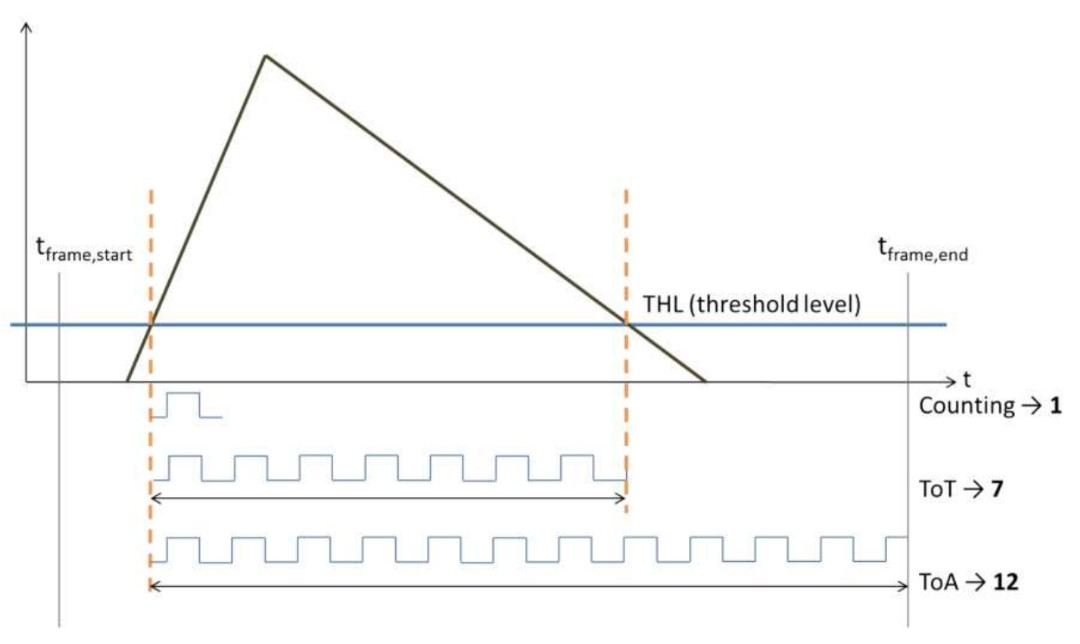
\includegraphics[scale=0.45]{modes.jpg}
	\caption{Digitální módy Timepix 2 \cite{Manek}} 
	\label{fig:modes}
\end{figure}	

Jakou energii interagující částice zanechala v senzoru můžeme zjistit z ToT měření. Počet hodinových cyklů odpovídá času, po který hodnota analogového napětí byla nad nastavenou detekovatelnou úrovní. Více o způsobu měření energie například viz. \cite{JAKUBEK2011S262}.

%TODO zminit ze countery mouhu ruzne kombinovat a zaroven jejich mody. PLUS zminit maskovani pixelu -> spotreba

\subsection{Komunikační rozhraní}
\subsubsection{Logické úrovně} 	% TODO nazev
\label{kap:3.2.1}
Timepix 2 umožňuje komunikaci po paraelním nebo sériovém datovém kanálu. Pro komunikaci přes paraelní bránu je možno využít 32 paraelních vodičů. Paraelní brána dosahuje násobně vyšších přenosových rychlostí, než sériový kanál, viz. obrázek \ref{fig:rychlosti}. Dosažením takovýchto rychlostí je zapotřebí na straně vyčítací elektroniky použít velmi rychlé rozhraní, například FPGA.  
\par Veškerá sériová komunikace probíhá po diferenciálních datových párech. Konkrétně se jedná o specifikaci SLVS \cite{SLVS}. Napěťové úrovně této specifikace lze najít na obrázku \ref{fig:SLVS_LVDS}. Jak lze na obrázku \ref{fig:SLVS_LVDS} vidět, specifikace SLVS je analogická se specifikací LVDS \cite{LVDS}. Výhody sériové komunikace jsou především v návrhu a spotřebě vyčítacího zařízení. Maximální datové rychlost, respektive rychlost komunikačních hodin je dle \cite{tpx2_manual} 100 Mhz. Lze tedy pro návrh použít například mikroprocesor. Hlavní nevýhodou sériové komunikace je oproti paraelní komunikaci vyčítací rychlost, která je násobně nižší \ref{fig:rychlosti}.
\begin{figure}[h!]
	\centering
	\captionsetup{justification=centering}
	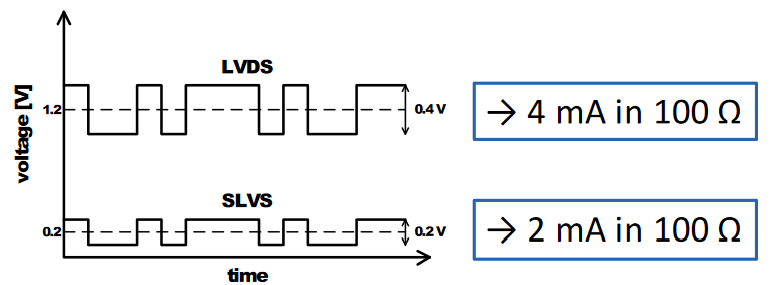
\includegraphics[scale=0.55]{SLVS_LVDS.png}
	\caption{SLVS specifikace \cite{SLVS}} 
	\label{fig:SLVS_LVDS}
\end{figure}	
\begin{figure}[h!]
	\centering
	\captionsetup{justification=centering}
	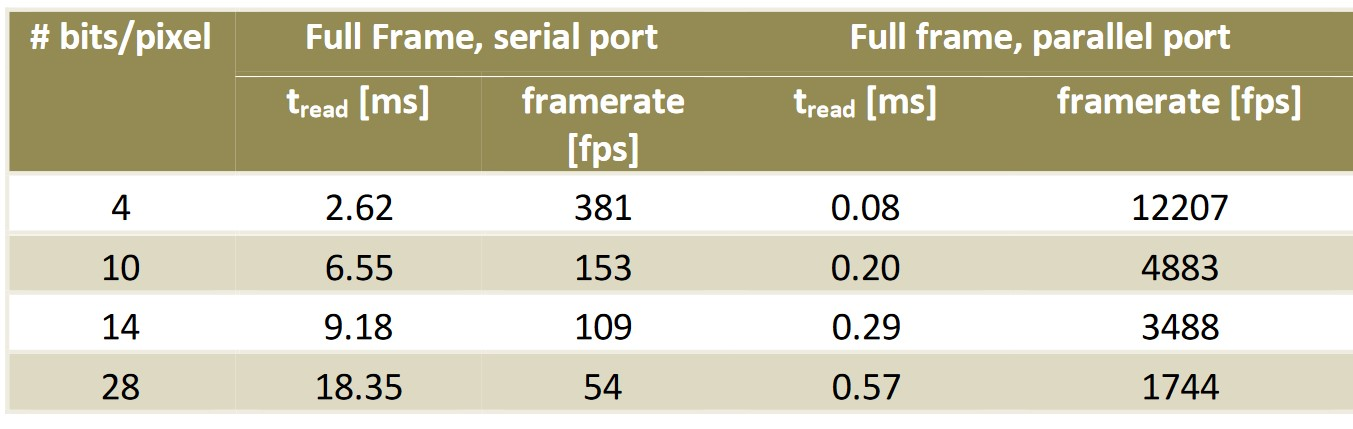
\includegraphics[scale=0.40]{rychlosti.jpg}
	\caption{Vyčítací rychlosti snímků z Timepix2. Frekvence hodin $f_{clock}$ = 100 MHz \cite{tpx2_manual}} 
	\label{fig:rychlosti}
\end{figure}	

\subsubsection{Struktura komunikace}
V této podkapitole bude popsána struktura komunikace s Timepix 2 za použití sériové komunikace popsané v \ref{kap:3.2.1}.  
%TODO popis signalu SPI pro TPX2 a casovani. Zminit i pakety SET/GET a jejich strukturu? 
Komunikace s Timepix 2 se rozděluje na příkazy SET a GET. Příkazy SET nastavujeme příslušný registr a příkazy GET daný registr vyčítáme. 
%TODO signaly potrebne pro komunikaci, ale pak i dac out atd ?.. 

%TODO MCLOCK
\subsection{Technická specifikace} %napáječky, kom. rozhraní, prikazy atd.., VN, hodiny pro měření, I/O piny
Timepix 2 je rozdělen do 256 x 256 pixelů. Rozteč mezi jednotlivými pixely je 55 $\mu$$m$. Celkově pak Timepix 2 má rozměry 16.6 x 14.14 mm. Vyčítací část detektoru tvoří ASCI chip navržen ve 130 nm CMOS technologii. Samotná výroba ASIC je zajišťována jedním z předních výrobců chipů, firmou TSMC \cite{TSMC} na Taiwanu. Všechny technické informace, nebude-li uvedeno jinak jsou čerpány z manuálu k detektoru Timepix 2 \cite{tpx2_manual}.

\subsubsection{Napájení}	
Timepix 2 ke své činnosti potřebuj celkem 3 napájení viz. tabulka \ref{tab:tpx2_napajeni}. Napájení VDD a VDDA slouží k napájení jádra Timepix 2, napájení VDDIO pak k napájení vstupních výstupních bran. Pokud chceme z Timepix 2 vyčíst CHIP ID, musíme na pin VDD33 aplikovat napájecí napětí 2.5 V. Při normální činnosti detektoru, je požadováno napětí 1.2 V. Celková spotřeba Timepix 2 při zapnutí všech pixelů a frekvenci datových hodin $f_{clock}$ = Mhz je dle \cite{Timepix2} nižší než 900 mW.
\begin{table}[h!]
	\centering
	\begin{tabular}{ |P{3cm}||P{5cm}|  }
		\hline
		\multicolumn{2}{|c|}{Napájecí úrovně Timepix 2} \\
		\hline
		Název pinu& Hodnota napájecího napětí [V] \\ \hline \hline 
		VDDIO & 2.5 \\ \hline		
		VDD & 1.2 \\ \hline 		 
		VDDA & 1.2 \\ \hline
		VDD33 & 2.5 (1.2)\\ \hline
	\end{tabular}
	\caption{Napájecí úrovně Timepix 2}
	\label{tab:tpx2_napajeni}
\end{table}
%TODO HV
\par Speciální kategorií napájení je napájení pro zajištění vysokého napětí, které se připojí na senzorovou vrstvu. Toto napětí zajistí vyprázdnění oblasti v polovodičové struktuře. Požadavky na parametry vysokého napětí záleží na typu a tloušťce senzorové vrstvy. Nejčastěji používaným materiálem senzorové vrstvy je křemík. Například vysoké velikost napětí použitá pro testování Timepix 2 se senzorovou vrstvou křemíku o tloušťce 500 $\mu$m dle \cite{Timepix2_500um} byla 100 V. Příklady velikosti vysokého napětí používaných pro křemíkové senzorové vrstvy lze najít v odkazech \cite{Timepix_500um_Pospisil}, \cite{Timepix_500um_Huston}. %TODO jiny material pro HV

\subsubsection{Rozhraní pro připojení Timepix 2 k desce plošných spojů}	% TODO nazev
Připojení Timepix 2 k desce plošných spojů je nejčastěji realizováno pomocí technologie \textit{wire bonding}. Timepix 2 má celkem 152 pinů pro přichycení wire bondů. Rozložení pinů je zobrazeno na obrázku \ref{fig:tpx2_floorplan} ve spodní části. Rozteč mezi jednotlivými plošky je 108 $\mu$m.
\begin{figure}[h!]
	\centering
	\captionsetup{justification=centering}
	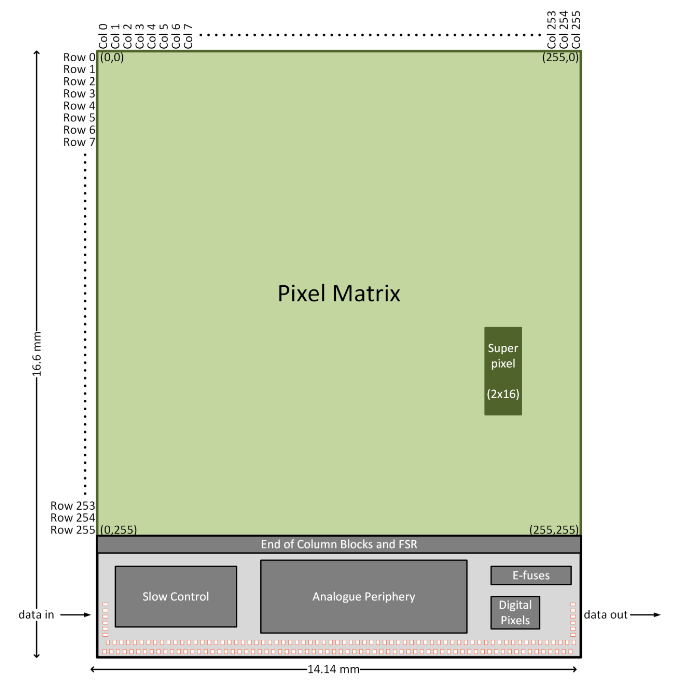
\includegraphics[scale=0.80]{tpx2_floorplan.png}
	\caption{Rozložení detektoru Timepix 2 \cite{tpx2_manual}} 
	\label{fig:tpx2_floorplan}
\end{figure}	
Dalším možným způsobem připojení Timepix 2 k desce plošných spojů je pomocí technologie zvané TSV. Respektive pomocí této technologie je možné signály vyvést ze zadní strany Timepix 2 k pájecím ploškám. Vznikne tím tak uspořádání, známe z technologie výroby pouzder BGA elektronických součástek. 
\par Běžnější způsob připojení Timepix 2 k desce plošných spojů je pomocí wire bondů. Použití wire bondů i technologie BGA je možné vidět na obrázku \ref{fig:bga}. Výhodou oproti technologii wire bondů je lepší praktické zacházení, díky absenci tenkých wire bondů, které jsou velmi náchylné na mechanické poškození. Další výhodou je poté technologicky méně náročné připojení detektoru. Avšak nevýhodou této technologie je vystavení chipu vysoké teplotě při pájení.
\begin{figure}[h!]
	\centering
	\captionsetup{justification=centering}
	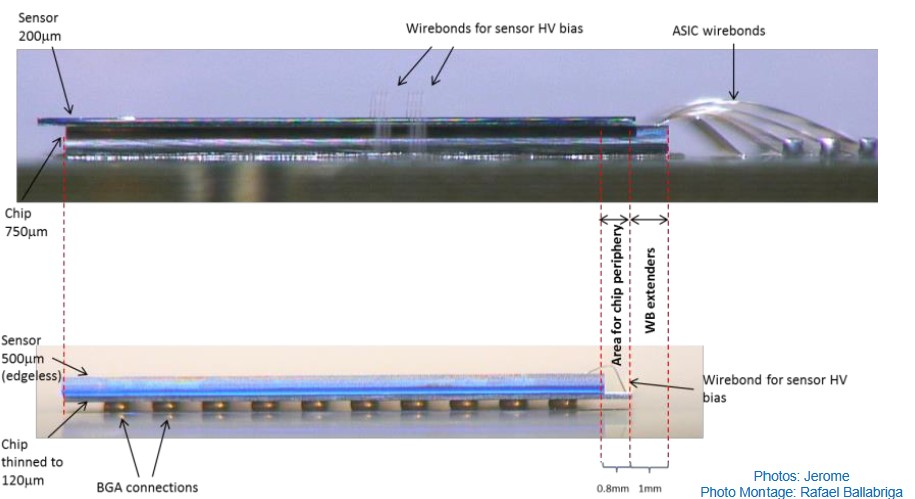
\includegraphics[scale=0.55]{bga.jpg}
	\caption{Připojení detektoru Timepix 2 k desce plošných spojů \cite{TSV}} 
	\label{fig:bga}
\end{figure}	









